\documentclass{resume} % Use the custom resume.cls style
\usepackage{graphicx}
\usepackage{wrapfig}
\usepackage[left=0.4 in,top=0.4in,right=0.4 in,bottom=0.4in]{geometry} % Document margins
\newcommand{\tab}[1]{\hspace{.2667\textwidth}\rlap{#1}} 
\newcommand{\itab}[1]{\hspace{0em}\rlap{#1}}
\name{Qian Xu} % Your name
\address{+86 15600616741 \\ drqianxu@163.com}  % Your phone number and email

\begin{document}

\begin{rSection}{Summary}

{7+ year work experience, focus on inference optimization on NPU/GPU including model compression/compilation optimization/performance modeling...}

\end{rSection}


\begin{rSection}{Education}

{\bf PHD of Electronics Engineering} \hfill {2013 - 2018}
\\ 
University of Chinese Academy of Sciences. Outstanding Graduates

{\textbf{Bachelor of Electronics Engineering}}  \hfill 2009 - 2013\\
Southeast University.


\end{rSection}

\begin{rSection}{Professional Experience}

\noindent



\textbf{Automotive Model Inference Optimization} \\ % Job title
\textit{AI Software Architect of Edge Computing Group} \hfill Alibaba PTG \hfill 2024-12 -- Present

\vspace{4pt}

Focused on inference acceleration and model optimization for in-vehicle AI workloads, targeting deployment on a custom GPGPU-based AI accelerator.

\begin{itemize}

\item \textbf{End-to-End Auto-Driving Model Inference Optimization}: 
Led the quantization, deployment, and operator-level optimization of multiple end-to-end models on custom GPGPU architecture.
\begin{itemize}
  \item Supported models including \textbf{VAD}, \textbf{Uni-AD}, \textbf{BEVFormer}, and \textbf{DiffusionDrive} with 8-bit quantization and $<$1\% open-loop accuracy drop.
  \item Developed optimized CUDA kernels for performance-critical ops including \textbf{DeformableAttention}/ \\ \textbf{GridSample}/\textbf{Voxelization}/\textbf{BevPoolv2}/\textbf{CoordTransformMatrix}/...
  \begin{itemize}
    \item Reducing latency to $\sim$1/6 of MMCV baseline.
  \end{itemize}
\end{itemize}

\item \textbf{VLM/VLA Inference Optimization}:
Worked on low-bit inference optimization and decoding acceleration for \textbf{Qwen-VL} and \textbf{Orion}.
\begin{itemize}
  \item \textbf{Qwen-VL} Quantization and Speculative Decoding:
  \begin{itemize}
    \item Experimented with \textbf{AWQ}, \textbf{SmoothQuant}, \textbf{GPTQ}, and \textbf{SpinQuant} to quantize Qwen-VL to \textbf{FP4} (weights + activations). Achieved higher accuracy than the W4A16 baseline through FP4 quantization, while reducing \textbf{Prefill} latency by 50\%.
    \item Integrated \textbf{Eagle} speculative decoding, achieving up to $\sim$4.7$\times$ decoding speedup.
  \end{itemize}
  \item \textbf{Orion} VLA model quantization:
  \begin{itemize}
    \item Combined quantization technique (\textbf{Spin + Scale + SVD decomposition + Mixed precision}) to retain accuray of FP4 model.
    \item Achieved $>$15\% latency reduction compared to FP8 baseline.
  \end{itemize}
  \item Conducted joint software-hardware evaluation of low-bit formats like \textbf{Microscaling FP4} and \textbf{NVFP4} to guide quantization hardware roadmap.

\end{itemize}

\end{itemize}


\textbf{NPU Software Architecture Design} \\ % Project or Role Title
\textit{AI Software Architect, Movidius NPU Team} \hfill Intel \hfill 2022-Q1 -- 2024-Q4

\vspace{4pt}

Contributed to the co-design of software and hardware architecture across multiple generations of Intel's Movidius NPU product line, focusing on compiler prototyping, advanced compilation techniques, and hardware/software co-optimization.

\begin{itemize}

\item \textbf{Prototype Compiler Development}:
Led the development of a prototype compiler to interface with backend hardware simulators for accurate and reliable model performance simulation.
\begin{itemize}
  \item \textbf{Hardware Change Validation}: 
  Evaluated the software stack impact of proposed hardware changes for future NPU generations. Integrated with hardware simulators to test architectural trajectories and identify those with improved PPA.
  
  \item \textbf{KPI Definition and Bottleneck Analysis}: 
  Defined key performance indicators using internal profiling toolsets. Analyzed performance bottlenecks in customer workloads (e.g., Microsoft, HP) to inform compiler feature planning and hardware evolution.
  
  \item \textbf{Model Coverage and Stability}: 
  Achieved support for over 800 models with 90\%+ coverage of Intel Open Model Zoo, ensuring broad compatibility and robustness.
\end{itemize}

\item \textbf{Advanced Compilation Technique Development}:
Explored cutting-edge compilation techniques to improve inference efficiency on NPUs. Collaborated with production compiler and DirectML teams to deliver transferable insights.
\begin{itemize}
  \item \textbf{LLM Performance Optimization}: 
  Optimized LLM inference through mixed precision, FlashAttention, task pipelining, and memory-efficient FFN tiling.
  
  \item \textbf{Tiling and Fusion}: 
  Developed automatic layer fusion algorithms for cross-component execution. Implemented double buffering for conflict-free scheduling.
  
  \item \textbf{Resource Allocation and Scheduling}: 
  Designed algorithms for efficient compute/memory resource allocation with reduced spilling. Developed prefetch scheduling to overlap communication and computation.
  
  \item \textbf{POC on Production Compiler}: 
  Implemented and validated proposed techniques on the MLIR-based production compiler targeting real-world software and hardware stacks.
\end{itemize}

\item \textbf{NPU Software-Hardware Co-Design}:
Actively participated in hardware definition and architectural exploration to ensure optimal SW/HW alignment for power, performance, and area (PPA).
\begin{itemize}
  \item \textbf{MAC Architecture}: 
  Evaluated trade-offs across MAC array size, SRAM bandwidth, PPE width, accumulator context size, and DSP instruction width.
  
  \item \textbf{Dynamism Support}: 
  Proposed and analyzed hardware support for dynamic shapes in transformers, enabling efficient MoE (Mixture of Experts) execution and flexible workload patching.
  
  \item \textbf{Interconnect Design}: 
  Defined tile interconnect strategies (unicast, multicast, broadcast) to balance latency, bandwidth, and scalability.
  
  \item \textbf{Memory Hierarchy Design}: 
  Contributed to memory subsystem design including size and placement of scratchpad SRAM, cache hierarchy, and DMA strategies.
\end{itemize}

\end{itemize}

\textbf{Model Compression for NPU} \\
\textit{Deep Learning software Engineer} \hfill Intel \hfill 2018-Q4 - 2022-Q1

\vspace{4pt}

Responsible for developing model compression algorithms for NPU. 
Leading the adoption and integration of state of the art model compression techniques including low-bit quantization/unstructured pruning/AutoML/NAS.

\begin{itemize}
\item \textbf{Low-bit quantization}:
Implementing state of the art model quantization techniques, including low-bit quantization methods like PACT and SAWB,  Mixed precision methods including HAQ and HAWQ, Unlinear quantization methods like log-based, outlier-aware and Squantizer. 

\item \textbf{Model pruning}: 
Implementing state of the art model pruning methods, including Sparse Momentum, Activation Map Compression, Auto Model Compression, Lottery Ticket and so on. 
Responsible for providing ultra compressed models for \textbf{MLPerf} inference, including \textbf{Resnet-50, Mobilenet, SSD-Mobilenet, SSD-Resnet34, Bert} and so on. 
Within 1\% top-1 accuracy drop of \textbf{Resnet-50}, achieved 84\% weight sparsity and 65\% activation sparsity, resulting in \textgreater 2$\times$ acceleration ratio compared to dense model.
\item \textbf{AutoML}: 
Implementing reinforcement learning based methods for model compression and provide innovative ideas to better compress the models. 
Developed a channelwise Hessian aware trace weighted quantization method, which outperforms state of the art methods by around 1\% top-1 accuracy.
\item \textbf{Network architecture search}: 
Network architecture search on NPU for better utilization of Hardware performance. Developed super-resolution network that is 6x faster than \textbf{EDSR} with ~7\% better PSNR. 
Also developed image classification network that is 10\% faster than \textbf{Mobilenet-V2} with ~5\% better accuracy top-1.
\end{itemize}


\textbf{Machine learning based Great Wall virtual repairing} \\
\textit{Machine Learning Engineer} \hfill Intel 2018-Q3 - 2018-Q4 
\begin{itemize}
\item \textbf{Use Machine learning for Great Wall restore} \\
- Cooperating with the Chinese Foundation for Cultural Heritage Conservation to launch an AI based method for its restoration. \\
- Use 3D-GAN to obtain the basic structure of the original Great Wall. Then use linear regression to fit the generated 3D-model with higher resolution. \\
- Expand the dimension of the brick images to include the structure-wise texture. Use GAN to generate the patterns of the missing part. \\
\end{itemize}

\textbf{The Institude of Chinese Academy of Sciences} \\
\textit{Post Graduate} \hfill 2013-Q3 - 2018-Q2



\begin{minipage}{0.75\textwidth}
    \begin{itemize}
    \item \textbf{Customized software design for proprietary WiFi chip}: Participated in the fabrication of two 802.11 chips, designed a customized MAC layer for the WiFi chip, and led WiFi authentication initiatives in accordance with the Ministry of Industry and Information Technology standards. Wrote the Linux driver from scratch for the WiFi chip and implemented the customized MAC layer.
    \item \textbf{Machine learning based SNR prediction}: Developed a machine learning-based method to enhance Signal-to-Noise Ratio (SNR) prediction in the MAC layer, resulting in a more than 20\% improvement in overall throughput compared to the original method. Additionally, implemented model compression techniques on the LSTM model, achieving better power efficiency and reduced latency.
    \end{itemize}
\end{minipage}
\hspace{0.04\textwidth}
\begin{minipage}{0.8\textwidth}
    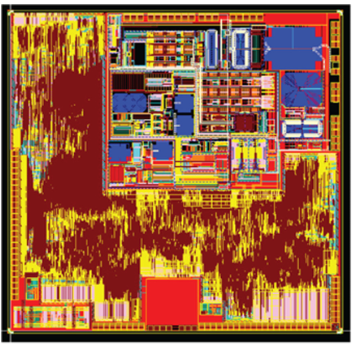
\includegraphics[width=0.2\linewidth]{./image.png}
\end{minipage}%


    
\end{rSection}

\begin{rSection}{Publications}{}
[1] \textbf{Xu Qian}, Victor Li, Crews Darren S, "Neural Architecture Search for Intel Movidius VPU", \textit{arxiv 2305.03739}

[2] \textbf{Xu Qian}, Victor Li, Crews Darren S, "Auto Hessian Aware Channel-wise Quantization of Neural Networks", \textit{6th Workshop on Energy Efficient Machine Learning and Cognitive Computing (EMC2 2020)}

[3] Charles Qi, Yi Wang, Hui Wang, Yang Lu, Shiva Shankar Subramanian, Finola Cahill, Conall Tuohy, Victor Li, \textbf{Xu Qian}, etc. "VPU-EM: An Event-based Modeling Framework to Evaluate NPU Performance and Power Efficiency at Scale", \textit{arxiv 2303.10271}

[4] \textbf{Xu Qian}, Bin Wu, Tianchun Ye, "QoS-aware A-MPDU retransmission scheme for 802.11 n/ac/ad WLANS", \textit{IEEE Communications Letters 21 (10), 2290-2293}

[5] \textbf{Xu Qian}, Bin Wu, Tianchun Ye, "Enhanced aggregation scheduler design in industrial 802.11 devices", \textit{Electronics Letters 53 (15), 1073-1075}

\end{rSection}

\begin{rSection}{Patents}{}
[1] Peiqing Jiang, Yuanyuan Li, \textbf{Xu Qian}, Haiyun Hong, Yinghao Li, "Executing Matrix Multiplication By Performing Convolution With Deep Neural Network Accelerator", Patent Filed, In Progress,  

[2] Yuanyuan Li, \textbf{Xu Qian}, Crews Darren S, Deepak Mathaikutty, Arnab Raha, Niall Hanrahan, Peiqing Jiang, "In-Place Execution Of Neural Network Operations With Scatter Write And Gather Read Across Memory Fragments", Patent Filed, In Progress

[3] Haiyun Hong, Yuanyuan Li, \textbf{Xu Qian}, Peiqing Jiang, Yinghao Li, "Reshaping Convolution Based On Configuration Of Deep Neural Network Accelerator", Patent Filed, In Progress

[4] \textbf{Xu Qian}, Yuanyuan Li, Crews Darren S, Zheng Qi, Deepak Mathaikutty, Raymond Sung, Arnab Raha, "Deep Neural Network Accelerator Facilitating Quantized Inference with Reduced Area and Power Consumption", patent filled, in progress

[5] \textbf{Xu Qian}, Haiyun Hong, Peiqing Jiang, Yuanyuan Li, Sijia Lou, "Apparatus, method, device and medium for accelerating computation of process engine", \textbf{WO2023092383A1}

[6] \textbf{Xu Qian}, Yuanyuan Li, Crews Darren S, "Apparatus and method for reinforcement learning based post-training sparsification", \textbf{WO2023082278A1}

[7] Crews Darren S, Yong Jiang, Yuanyuan Li, \textbf{Xu Qian}, Peiqing Jiang, Haiyun Hong "Methods and apparatus to accelerate convolution" \textbf{WO2023044707A1}

[8] Haiyun Hong, Umer lftikhar Cheema, Peiqing Jiang, Yuanyuan Li, Deepak Mathaikutty, \textbf{Xu Qian}, Arnab Raha, "PrepNN: Activation function-based preprocessor for compiler to enhance the Accuracy and	Performance of Neural Networks on an Al accelerator", Patent Filed, In Progress 

[9] Yuanyuan Li, \textbf{Xu Qian}, Deepark Mathaikutty, Arnab Raha, Haiyun Hong, "A method to Reduce Workload Overhead for LLM Execution on resource constrained DNN Accelerators", Patent Filed, In Progress 
\end{rSection}

\end{document}

